%%%%%%%%%%%%%%%%%%%%%%%%%%%%%%%%%%%%%%%%%%%%%%%%%%%%%%%%%%%%%%%
%
% Welcome to Overleaf --- just edit your LaTeX on the left,
% and we'll compile it for you on the right. If you open the
% 'Share' menu, you can invite other users to edit at the same
% time. See www.overleaf.com/learn for more info. Enjoy!
%
%%%%%%%%%%%%%%%%%%%%%%%%%%%%%%%%%%%%%%%%%%%%%%%%%%%%%%%%%%%%%%%
\documentclass[11pt, nopagenumbers]{adamblan-hw}

\newcommand{\questionBanner}[1]{%
    \vspace{.25in} \hrule \vspace{0.4em}%
    \noindent{\bf\arabic{questionCounter}: #1}%
    \vspace{0.8em} \hrule \vspace{.10in}%
    \addtocounter{questionCounter}{1}%
}

% Some frequently helpful commands. Feel free to add more of your own.
\newcommand{\NN}{\mathbb{N}}
\newcommand{\ZZ}{\mathbb{Z}}
\newcommand{\QQ}{\mathbb{Q}}
\newcommand{\RR}{\mathbb{R}}

\newcommand{\limit}{\lim\limits}
\newcommand{\limn}{\limit_{n \to \infty}}

% usage \set{1, 2, 3} for {1, 2, 3}. Will automatically resize the braces too.
\newcommand{\set}[1]{\left\{ #1 \right\}}
% usage \abs{\frac{1}{2}} for |1/2|. Will automatically resize the bars too.
\newcommand{\abs}[1]{\left| #1 \right|}
% same as \abs but with double bars like for vector magnitude
\newcommand{\norm}[1]{\left\| #1 \right\|}
% usage \ceil{\frac{1}{2}} for \lceil 1/2 \rceil. Will automatically resize the bars too.
\newcommand{\ceil}[1]{\left\lceil #1 \right\rceil}
% usage \floor{\frac{1}{2}} for \lfloor 1/2 \rfloor. Will automatically resize the bars too.
\newcommand{\floor}[1]{\left\lfloor #1 \right\rfloor}
% usage \round{\frac{1}{2}} for \lfloor 1/2 \rceil. Will automatically resize the bars too.
\newcommand{\round}[1]{\left\lfloor #1 \right\rceil}
% The following commands are defined via the xparse package, which you can look up for more info if you want.

% \par(\frac{1}{2}) will automatically resize the parenthesis
\NewDocumentCommand{\paren}{r()}{\ensuremath{\left( #1 \right)}}
% \brac[\frac{1}{2}] will automatically resize the brackets
\NewDocumentCommand{\brac}{r[]}{\ensuremath{\left[ #1 \right]}}

\usepackage{graphicx}
\graphicspath{ {./images/} }

%%%%%%%%%%%%%%%%% Identifying Information %%%%%%%%%%%%%%%%%
%% DO NOT INCLUDE YOUR NAME ANYWHERE IN THE PDF. WE WANT %%
%% TO GRADE ANONYMOUSLY TO AVOID BIAS!!!!                %%
%%%%%%%%%%%%%%%%%%%%%%%%%%%%%%%%%%%%%%%%%%%%%%%%%%%%%%%%%%%

\begin{document}

\begin{question}{Deriving Naive Bayes}

% (a) - Proportional value of P(A | B)
\begin{part}
Since we're just trying to broadly compare $P(spam)$ vs. $P(not \ spam)$ to classify
the document, we note that dividing by $Pr(B)$ simply scales down the values.
We just need the result of comparing $P(spam)$ to $P(not \ spam)$, so as long as the proportional
proporitional value maintains the truth value of the inequality, we don't need to calculate the exact value.
Note that since $B$ is drawn from some ideal distribution as well, we're scaling both probablities
down by the same factor which doesn't change the truth value of the inequality, so it is 
sufficient for us to just calculate the proporitional values. 
\end{part}    

\end{question}

\begin{question}{Uh oh! Underflow}

% (a) - Smallest representable floating point number
\begin{part}
The smallest representable representable floating point number is $5 * 10^{-324}$.
This value was calculated by writing a Python script that initializes a float value
and continually divides that number by $2$ till it reaches  $0.0$. The result of 
each division is stored. The reason why this works is because dividing by 2 is equivalent
to \texttt{num >> 1}, so eventually, only the last bit in $num$ will be set which will give
us the smallest representable floating point number.

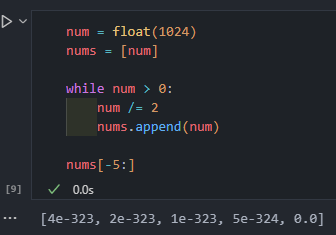
\includegraphics{1a.png}

\end{part}

\pagebreak
% (b) - Floating point arithmetic is not associative
\begin{part} 
To prove that there exists three floating point numbers $x, y, z$ where
$x + (y + z) = (x + y) + z$ where $+$ is floating point addition, it's sufficient
to simply find one such example. As the below code demonstrates, if $x = 0.1$, 
$y = 0.2$, and $z = 0.3$, then their addition is not associative.

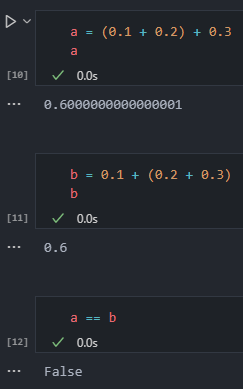
\includegraphics{1b.png}
\end{part}

\pagebreak
% (c) - Smallest normal FP
\begin{part}
To find the smallest normal number greater than 0, all we need to do is
work through each part of the expression for a normal number and minimize it,
and since all the parts are being multiplied, minimizing each part minimizes
the product.

Recall that if $e \neq 0$ or $e \neq$ \texttt{0x7ff}, then a number is "normal" and
is represented by $$(-1)^s * 2^{e-1023} * (1 + \sum\limits_{i=1}^{52}{b_{52-i}2^i})$$ 

Since the number has to be greater than 0, $s$ must be 0. 

The second portion of $2^{e-1023}$ is minimized when $e = 1$. By the pre-conditions
of a normal number and the number of bits allocated for $e$
, $e = \{e \in \ZZ | 1 \leq e \leq 2046\}$. To minimize this portion, we need the exponent
to be minimized, and this occurs when $e = 1$.

For the last porition $(1 + \sum\limits_{i=1}^{52}{b_{52-i}2^i})$, it's easy to see
that if the entire summation is set to 0 (achieved by setting all the fraction bits to 0),
then the quantity is minimized. 

As such, the smallest normal number greater than 0 is 
$$(-1)^0 * 2^{1-1023} * (1 + 0) = \fbox{$\frac{1}{2^{1022}}$}$$ 
\end{part}

\pagebreak
% (d) - How many representable values between 0 and 1
\begin{part}
We calculate this by starting
with pre-conditions for both categories and the expressions for them and counting
how many values are there.

We start with normal numbers. 

Recall that if $e \neq 0$ or $e \neq$ \texttt{0x7ff}, then a number is "normal" and
is represented by $$(-1)^s * 2^{e-1023} * (1 + \sum\limits_{i=1}^{52}{b_{52-i}2^i})$$ 

By the preconditions of "normal" numbers and the
number of bits allocated for $e$, $e = \{e \in \ZZ | 1 \leq e \leq 2046\}$.

Since our number must be greater than 0, our expression simplifies to 
$$2^{e-1023} * (1 + \sum\limits_{i=1}^{52}{b_{52-i}2^i})$$ 

Note that the second term
of the product is always greater than $1$, so to get all values less than $1$, the first
term of the product must be less than $1$. This is accomplished when $e - 1023 < 0$, so 
so $e < 1023$. Our choices for $e$ are now restricted to $e = \{e \in \ZZ | 1 \leq e \leq 1022\}$.

Since there are $1022$ choices for $e$ and $2^{52}$ choices for the $f$ (the second
term of the product is the decimal value of the fraction in the floating point number, and
there are $52$ bits allocated for the fraction with the choice of either $0$ or $1$), we
can apply the rule of product to get the total number of "normal" numbers in $(0, 1)$ is 
$1022 * 2^{52}$.

For subnormal numbers, a very similar process applies. Since the number must be positive, $s = 1$,
and our expression becomes $$2^{-1022} * \sum\limits_{i=1}^{52}{b_{52-i}2^i}$$ To calculate
the number of choices we have for $f$, we note that the maximum value of $f$ is $1 - \frac{1}{2^{52}}$, 
and it's easy to see that $max(subnormal) = 2^{-1022} * max(f) = 2^{-1022} * (1 - \frac{1}{2^{52}})$ is always less than $1$, 
and since all choices of $f$ are less than $max(f)$, all choices of $f$ except $0$ by the exclusion of $0$
in our domain, are valid. As such, there are $2^{52} - 1$ choices for $f$ and thus 
$2^{52} - 1$ subnormal numbers that can be represented in $(0, 1)$. 

Now, we can just sum the number of normal and subnormal value to get the total number of values.
$$\#(values) = \#(normal) + \#(subnormal) = 1022 * 2^{52} + 2^{52} - 1 = \fbox{$1023*2^{52} - 1$}$$
\end{part}

\pagebreak
% (e) - How many representable values in the range (-\infty, 0)
\begin{part}
We calculate this by starting
with pre-conditions for both categories and the expressions for them and counting
how many values are there.

We start with normal numbers. 

Recall that if $e \neq 0$ or $e \neq$ \texttt{0x7ff}, then a number is "normal" and
is represented by $$(-1)^s * 2^{e-1023} * (1 + \sum\limits_{i=1}^{52}{b_{52-i}2^i})$$ 

By the preconditions of "normal" numbers and the
number of bits allocated for $e$, $e = \{e \in \ZZ | 1 \leq e \leq 2046\}$.

Since our number must be less than 0, $s=-1$, and our expression simplifies to 
$$-2^{e-1023} * (1 + \sum\limits_{i=1}^{52}{b_{52-i}2^i})$$ 

Note that the second term
of the product is always positive, so since we're multiplying it by a negative number,
the value will always be negative regardless of our choice of $e$ or $f$. There are 
$2046$ choices for $e$ and $2^{52}$ choices for $f$, by the law of product, there are $2046 * 2^{52}$ normal 
values that can be respresented in $(-\infty, 0)$

For subnormal numbers, a very similar process applies. Since the number must be negative, $s = -1$,
and our expression becomes $$-2^{-1022} * \sum\limits_{i=1}^{52}{b_{52-i}2^i}$$ To calculate
the number of choices we have for $f$, we note that the maximum value of $f$ is $1 - \frac{1}{2^{52}}$, 
and it's easy to see that $max(subnormal) = -2^{-1022} * max(f) = -2^{-1022} * (1 - \frac{1}{2^{52}})$ is always less than $0$, 
and since all choices of $f$ are less than $max(f)$, all choices of $f$ except $0$, by the exclusion of $0$
in our domain, are valid. As such, there are $2^{52} - 1$ choices for $f$ and thus 
$2^{52} - 1$ subnormal numbers that can be represented in $(-\infty, 0)$. 

Now, we can just sum the number of normal and subnormal value to get the total number of values.
$$\#(values) = \#(normal) + \#(subnormal) = 2046 * 2^{52} + 2^{52} - 1 = \fbox{$2047*2^{52} - 1$}$$
\end{part}

\pagebreak
% (f) - log(x) is increasing
\begin{part}
Lemma: \textbf{For a continuous function $f(x)$ with a domain of $(0, \infty)$, if $f'(x) > 0$ for all $x$ on that domain,
then $f(x)$ is increasing.}

\begin{proof}
We start by assuming the left that $f'(x) > 0$ for all $x$ in $(0, \infty)$ and proceed with contradiction.

Let's assume there is some arbitrary interval $I$ in the domain of $f(x)$ with endpoints $(a, b)$ where 
$f(x)$ is decreasing. Since $a < b$, by the definition of a decreasing function, we can say that
$f(a) > f(b)$ which is equivalent to $f(b) - f(a) < 0$. 

Since $f$ is diffentiable on $(a, b)$ and continuous on $[a, b]$, there exists a $c \in (a, b)$ such that
$$f'(c) = \frac{f(b) - f(a)}{b - a}$$

Since $f(b) - f(a) < 0$ and $b - a > 0$, $f'(c)$ is negative. This contradicts the condition
that $f'(x)$ is positive for all $x$ in $(0, \infty)$. As such, our original assumption that $I$ is decreasing
must be false and $f(x)$ must be increasing over $I$. $f(x)$ can't be constant over $I$ because
applying the MVT to that interval would result in $f(x)=0$ which also contradicts our pre-condition.
As such, since we have proven that $f(x)$ is increasing 
over any arbitrary interval $I$, $f(x)$ must be an increasing function over the entire domain.
\end{proof}

Note that $f(x) = ln(x)$ is a continuous function with a domain of $(0, \infty)$ and 
$f'(x) = \frac{1}{x}$ is greater than $0$ for all $x$ in $(0, \infty)$, so by the lemma proven above,
$f(x) = ln(x)$ must be an increasing function.
\end{part}

% (g) - Taking log increases representable numbers
\begin{part}
Note that when we compute the $ln(x)$ for an $x \in (0, 1)$, the output is in
the range $(-\infty, 0)$. From part d and e, we know that we can represent almost twice
as many values over $(-\infty, 0)$ as compared to $(0, 1)$. As such, if we take the $log$
of the probability which is defined over $(0, 1)$, then we can nearly double the number of
probablities we can represent.
\end{part}

% (h) - Log must be monotonic
\begin{part}
When transforming our probablity, we need to ensure that the relativity of the probablities
is maintained i.e. if $a < b$, then $f(a) < f(b)$ and if $a > b$, then $f(a) > f(b)$ for all $a, b$. This is the definition
of monotonicity. If our transformation function isn't monotonic,
then the relativity of the probablities won't
be maintained.
\end{part}

\end{question}

\questionBanner{Implement Naive Bayes}
% SUBMIT YOUR CODE FOR 2 IN THE OTHER SUBMISSION ON GRADESCOPE
% INCLUDE YOUR RESULTS ON EMAILS AND TWEETS HERE
\begin{verbatim}
The results of my code were as follows:

Counter({`negative': 1166, `positive': 780})
Counter({`positive': 420, `negative': 216})
Counter({`ham': 323, `spam': 145})
Counter({`ham': 32})
\end{verbatim}

\end{document}